%!TEX root = ../../super_main.tex
\part{Second Sprint}
\label{par:second_sprint}

\chapter{Sprint Overview}
\label{sec:sprint2_overview}
The focus of the second sprint was to complete and stabilize the applications with the highest assigned priority, the priorities are listed in \tabref{tab:application_priorities_sprint_two}, which was determined with the customers. The costumers were asked to prioritize the list of existing applications, with 0 being the highest priority, during the Sprint Planning Meeting for the second sprint. Application responsibilities were then divided among the GUI-groups. Some applications do not have a priority because the customers could not relate to these.

\todo{Write intro what will be described in this chapter.}

\begin{table}[!htbp]
	\center
    \begin{tabular}{l l}
        \textbf{Application}     & \textbf{Priority} \\ \hline\hline
        \launcher                & 0                 \\ \hline
        \emph{Picto Search}      & 1                 \\ \hline
        \emph{Week Schedule}     & 2                 \\ \hline
        \emph{Sequence}          & 3                 \\ \hline
        \emph{Picto Creator}     & 4                 \\ \hline
        \ct                      & 5                 \\ \hline
        \emph{Picto Reader}      & 6                 \\ \hline
        \emph{Timer}             & 6.5               \\ \hline
        \emph{Life Story}        & 7                 \\ \hline
        \emph{Category Game}     & 8                 \\ \hline
        \emph{Voice Game}        & 9                 \\ \hline
        \emph{Profile Manager}   & 10                \\ \hline
        \emph{Web admin}         & -                 \\ \hline
        \gc         		     & -                 \\ \hline
    \end{tabular}
    \caption{Application priorities}
    \label{tab:application_priorities_sprint_two}
\end{table}

\FloatBarrier

We did not really have any project preferences for this sprint, since we already brought the \launcher to a stable state. The \giraf \ct was given a high priority at the Sprint Planning Meeting for the second sprint, and we got assigned to this project since we did not have any preferences. 

\section{Category Tool and Components}
\label{sec:category_tool_and_components}

The \giraf \ct is an application which is used by guardians to create and manage pictogram categories. These categories are used across many different applications, for instance the \emph{Category Game} application also known as \emph{Train}.
\\\\
We were also assigned to construct a series of standard components for the \gc library. These standard components should, as of the start of the second sprint, include: A specialization of the Android \androidinline{ActionBar} for \giraf, buttons with automatically scaling text, and a standard dialog to use across all applications.

%!TEX root = ../../super_main.tex
\section{Initial Thoughts}

The \ct was in an unstable state and could not even compile when this group inherited it. The \ct does not conform to many general design principles and crashes on a regular basis. This section describes the design problems and some bugs with the \ct as it was inherited. A screenshot of the \ct as it looked once we brought it to a compilable state can be seen in \figref{fig:category_tool_old}. The reader is invited to reference \figref{fig:category_tool_old} while reading this section.

\begin{figure}[!htbp]
    \centering
    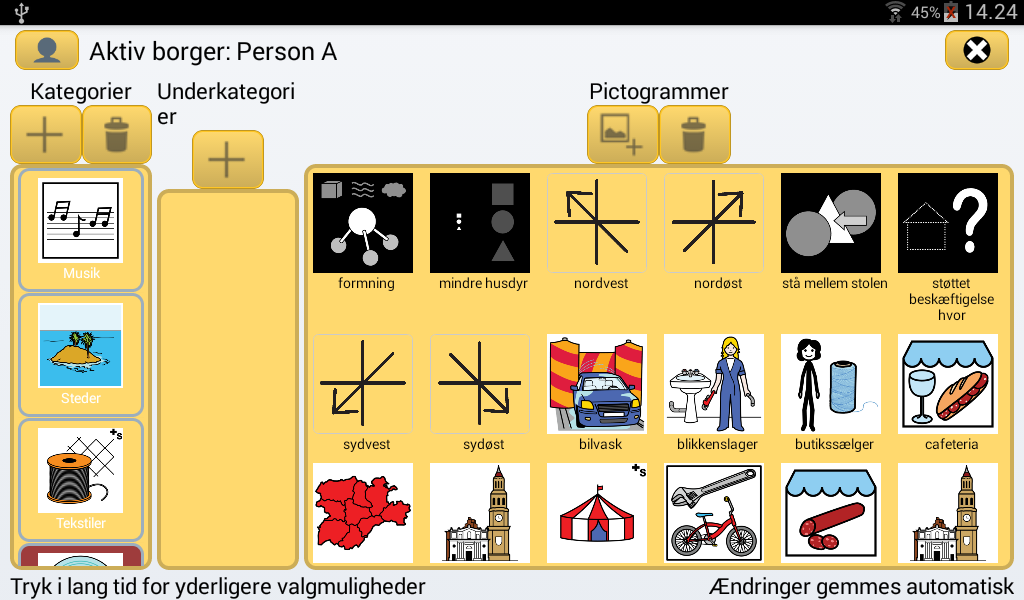
\includegraphics[width=\textwidth]{sprint_two/initial_category_tool}
    \caption{Old \ct}
    \label{fig:category_tool_old}
\end{figure}

\subsection{Interaction Design}

There is too much functionality on the same single screen in the current state of the \ct. Creation and modification of categories, sub-categories, adding and removing pictograms from categories is all done on the same screen which leaves little screen estate for each function.  

\subsubsection{Buttons}

The \ct includes non standardized buttons of different sizes and shapes. Buttons with square icons have different rectangular shapes. The buttons are too small in general and can be difficult to click. There is no margin between buttons which makes it easy to miss-click grouped buttons. The different buttons, and other widgets in general, in the \ct are not aligned very well. There are a couple of different contextual buttons that only appear once pictograms or categories are selected. 

\subsubsection{Android Design Guidelines}

The Android design guidelines have changed and now advices to exclusively use long press action for multiple selection in lists. Long press is currently used to show a contextual menu for categories where it is possible to change the title, color, and icon of the category and to copy it. It is currently not possibly to perform multiple selection of pictograms. 

\subsubsection{Selection}

There is no visual cues of selection anywhere in the \ct. It is not possible to determine the currently selected category from the list of categories. This is a problem for the contextual delete button for categories. The contextual delete button for categories deletes the currently selected category but the only way to determine the current category is from the pictograms displayed to the right in the current selected category. 

\subsection{Crashes}

The application crashes when there are too many pictograms in a category and the user scrolls too far down in the list. 

\subsection{Explanatory Text}

There is cluttering explanatory text in the bottom of the screen which does not really help. The purpose of this explanatory text was to to reveal hidden features in the application, such as telling the user to long press certain items for a contextual menu to appear, which is also against the Android Guidelines \parencite{android_guidelines_longpress}.

\subsection{Pop-up Windows}

There is multiple contextual pop-ups in the application, for instance when creating a new category. Other pop-ups appears on top of the category creation pop-up when, for instance, the user neglects to provide a name when creating a new category. Pop-ups on pop-ups is not very good practice.  

There is another problem with the pop-ups. The pop-ups creates an overlay on top of the remaining background only this overlay does not disappear when they are closed using the Android soft- or hardware- back button instead of their cancel button. 
 
\subsubsection{Monkey Tests}
\todo{insert stuff about monkey test}


%!TEX root = ../../../super_main.tex

\chapter{Issues and Solutions}

\todo[inline]{Write introduction}

%!TEX root = ../../../super_main.tex
\section{Restructuring Issues}
\label{sec:restructuring_issues}

During the first sprint, a lot of changes to the Git submodule structure were introduced by a \emph{Build and Deployment} group of the multiproject. These changes include changing a lot of submodule dependencies, changing namespaces for submodules, and changing library dependencies. \todo{DONE-start(home): forklar hvad gradle er} The library dependencies is handled using the open source automation builder called Gradle \parencite{gradle} which is a standard build script in the Android Studio IDE. \todo{DONE-end(home)} After the aforementioned changes had been implemented for the submodule structure, it had not been enforced in all of the \giraf projects who implemented the submodules. Because of this, many unforeseen issues had been introduced to the system, hereunder mismatches between project structure, \mono{gradle.build} files and \mono{gradle.settings} files, and furthermore git issues related to referring to old versions of submodules. Partially due to these changes, the \ct was unable to build and run on any Android device, and we therefore had to spend a lot of time and resources on addressing these issues. 
\\\\
After fixing all the problems related to the \ct, we talked to the other groups of the GUI subproject, who told us that some of them have parts of the same issues that we have already found solutions for. We therefore decided to dispatch one member of our group to the other groups, such that they would also be able to progress with their development. This of course results in reduced resources for our own group for a period of time, which most likely results in reduced productivity at the end of the sprint, but we weigh the general progress of the multiproject higher than our own progress.
\\\\
Later in the sprint, it was discovered that some of the changes we had to make to the submodule structure of the project, in order to make the \ct compile and work, were actually something that one of the database groups had been working on. We therefore worked together with this database group in order to restore the project to a working state where their necessary components were also present. Even later, this change also proved futile, since the \emph{Build and Deployment} sub-project had been working on making the confusing submodule structure into online libraries instead. 

\todo{Skriv at det havde været bedre at få en build and deployment til at gøre det for os.}

%!TEX root = ../../../super_main.tex

\section{\giraf Components issues}

This group was responsible for the further development of cross project \giraf Components as described in \secref{sec:sprint2_overview}. More components were suggested during the second sprint and new components were developed to replace old components. The development of these components are described in this section. Old components were marked as deprecated with the \androidinline{@Deprecated} annotation when new components replaced old ones.  

%!TEX root = ../../../super_main.tex
\subsection{GirafActivity and ActionBar}
\label{sec:giraf_activity_actionbar}

One of the user stories was to get a top-bar, called \androidinline{ActionBar} in Android, in all applications with a back-button for navigation between applications and their activities. A developerstory, which said that there should be build a common \androidinline{ActionBar} for use across all sub-projects, was created on the basis of this user story. The implementation of the new \giraf \androidinline{ActionBar} is described in this section. A shortened version of this section was published on the \giraf Redmine \parencite{redmine} forum.

\subsubsection{Idea and Implementation}

The idea of the new \androidinline{ActionBar} is that it should include a centered title of the current activity and two dynamic rows of \giraf buttons, in which the client of the \androidinline{ActionBar} should be able to add buttons, while always having a back-navigation-button in the upper leftmost corner. This back-navigation-button should have the same behavior as the Android ``hardware-back-button''.

The new \androidinline{ActionBar} was implemented by subclassing the Android \androidinline{Activity}, with a class called \androidinline{GirafActivity}, and by creating two new Android application themes called \androidinline{GirafTheme} and \androidinline{GirafTheme.NoTitleBar}. The idea is then that all activities across all projects should subclass \androidinline{GirafActivity} and thereby get the customizations of the \androidinline{ActionBar}. Clients of \androidinline{GirafActivity} should then for each \androidinline{GirafActivity}, in their \androidinline{AndroidManifest.xml} file, specify if they want an \androidinline{ActionBar} or not by specifying either \androidinline{GirafTheme} or \androidinline{GirafTheme.NoTitleBar} as their theme.

%  Snak om linearlayouts
The custom \androidinline{ActionBar} is implemented using a custom layout, an Android \androidinline{RelativeLayout}, for the \androidinline{ActionBar}. The \androidinline{RelativeLayout} then contains a centered \androidinline{TextView} for the title and a back-\androidinline{GirafButton} placed at the leftmost position in the \androidinline{ActionBar}. A \androidinline{LinearLayout} is then placed to the right of the back-button and another \androidinline{LinearLayout} is placed to the right of the title; both with the purpose of containing \androidinline{GirafButton} instances added by the client of the \androidinline{GirafActivity} i.e. the client of the customized \androidinline{ActionBar}. 

\subsubsection{GirafActivity API}

The \androidinline{GirafActivity} provides an easy API for adding \giraf buttons, i.e. instances of the \androidinline{GirafButton} class, to its customized \androidinline{ActionBar} through a method called \androidinline{addGirafButtonToActionBar}. \androidinline{addGirafButtonToActionBar} takes two arguments; one being a \androidinline{GirafButton} and the other a flag which is either \androidinline{GirafActivity.LEFT} or \androidinline{GirafActivity.RIGHT}. The \androidinline{GirafButton} is then added to the leftmost position of the title, and to the right of the back-button, if the \androidinline{GirafActivity.LEFT} flag is used or conversely to the right of title if the \androidinline{GirafActivity.RIGHT} flag is used. 
The default behavoir of the back-navigation-button in the \androidinline{ActionBar}, which is to \androidinline{finish} the current \androidinline{Activity}, can be changed by overriding the \androidinline{onBackPressed} method of the corresponding \androidinline{GirafActivity}.          


%!TEX root = ../../../super_main.tex
\section{Consistent Dialogs}
\label{sec:consistent_dialogs}

During the spring the dialog have gotten a major overhaul. The dialog implemented, from previous years (\androidinline{GDialog} see FIGREF) was found to be inconsistent with the design manual. It was wanted that all dialogs and pop-ups in the \giraf-software suite was replaced with something consistent. This was done by implementing an abstract \androidinline{GirafDialog} which enables a lot of functionality for the dialogs used

%!TEX root = ../../../super_main.tex
\section{Improved Design of the \emph{Category Tool}}
\label{sec:improved_design}
We decided to make a major rework of the current design of the \ct. The new design must be an improvement to the old design, and should not suffer from the same design flaws. Furthermore, the new design should improve usability and should ideally never crash when used. Besides this, the tool should not implement any unwanted features, such as colored categories or sub categories.
\\\\
Instead of just implementing an incremental design straight ahead, some initial markup of the design, which has gone through some iterations, has been made. This markup is then later used in the implementation of the design. Different parts of this markup are described throughout this section.

\subsection{Separation of Categories by Type}
The customers have previously described that they would like to be able to copy categories between citizens. To accommodate this, it was decided that categories must be ``bound'' to an institution instead of actual citizens. This will ensure that the categories for a specific institution are independent of any citizen. When a category is assigned to a citizen, the content (pictograms) should be copied to a new category (with the same name) which then belongs to the citizen. This will allow guardians to make changes to a specific citizen-assigned category without affecting other categories. 
\\\\
Take for instance an institution that have the category \emph{Toys} which has some pictograms associated with it. The guardians of this institution then decide that citizens \emph{A} and \emph{B} should have access to use this category, therefore they copy the \emph{Toys} category to both citizens. However, \emph{A} is unsatisfied with the new category and feels that it is missing his favorite toy. To make \emph{A} happy, the guardians then add a pictogram of his toy to \emph{A}'s category. Because of the way the system is designed, this action should have no effect on the the \emph{Toys} category of \emph{B}.
\\\\
This idea of separating categories into institution and citizen-assigned categories can be difficult to understand for new users, so it will require the user-interface to be clear about which categories are being viewed or modified. Therefore, when using the \ct the user should always be aware of what type of categories are being presented.
\\\\
Clarification as to where the user currently is in the \ct should be indicated by use of the \androidinline{ActionBar} mentioned in \secref{sec:giraf_activity_actionbar}. This bar should clearly state whose categories are shown at the moment.

\subsection{Home Screen}
\label{sec:home_screen}
When opening the \ct, the user should be presented with a screen similar to the markup seen in \figref{fig:improved_design_launch_screen}. As seen in the figure, the user is presented with a list (to the left). This list contains all of the categories that are bound to the specific institution, based on the affiliation of the currently logged in guardian. On the right side of the screen, the user is presented with a small introduction to the tool. For instance, the arrow-text reads \translated{Vælg en kategori for at se dens indhold}{Choose a category to see its content}. This will help to user to understand that the left-side contains categories, and that they are clickable. On the right, the user is also presented with two buttons, namely \translated{Opret ny kategori}{Create new category} and \translated{Administrer borgere}{Administrate citizens}.

\begin{figure}[!htbp]
    \centering
    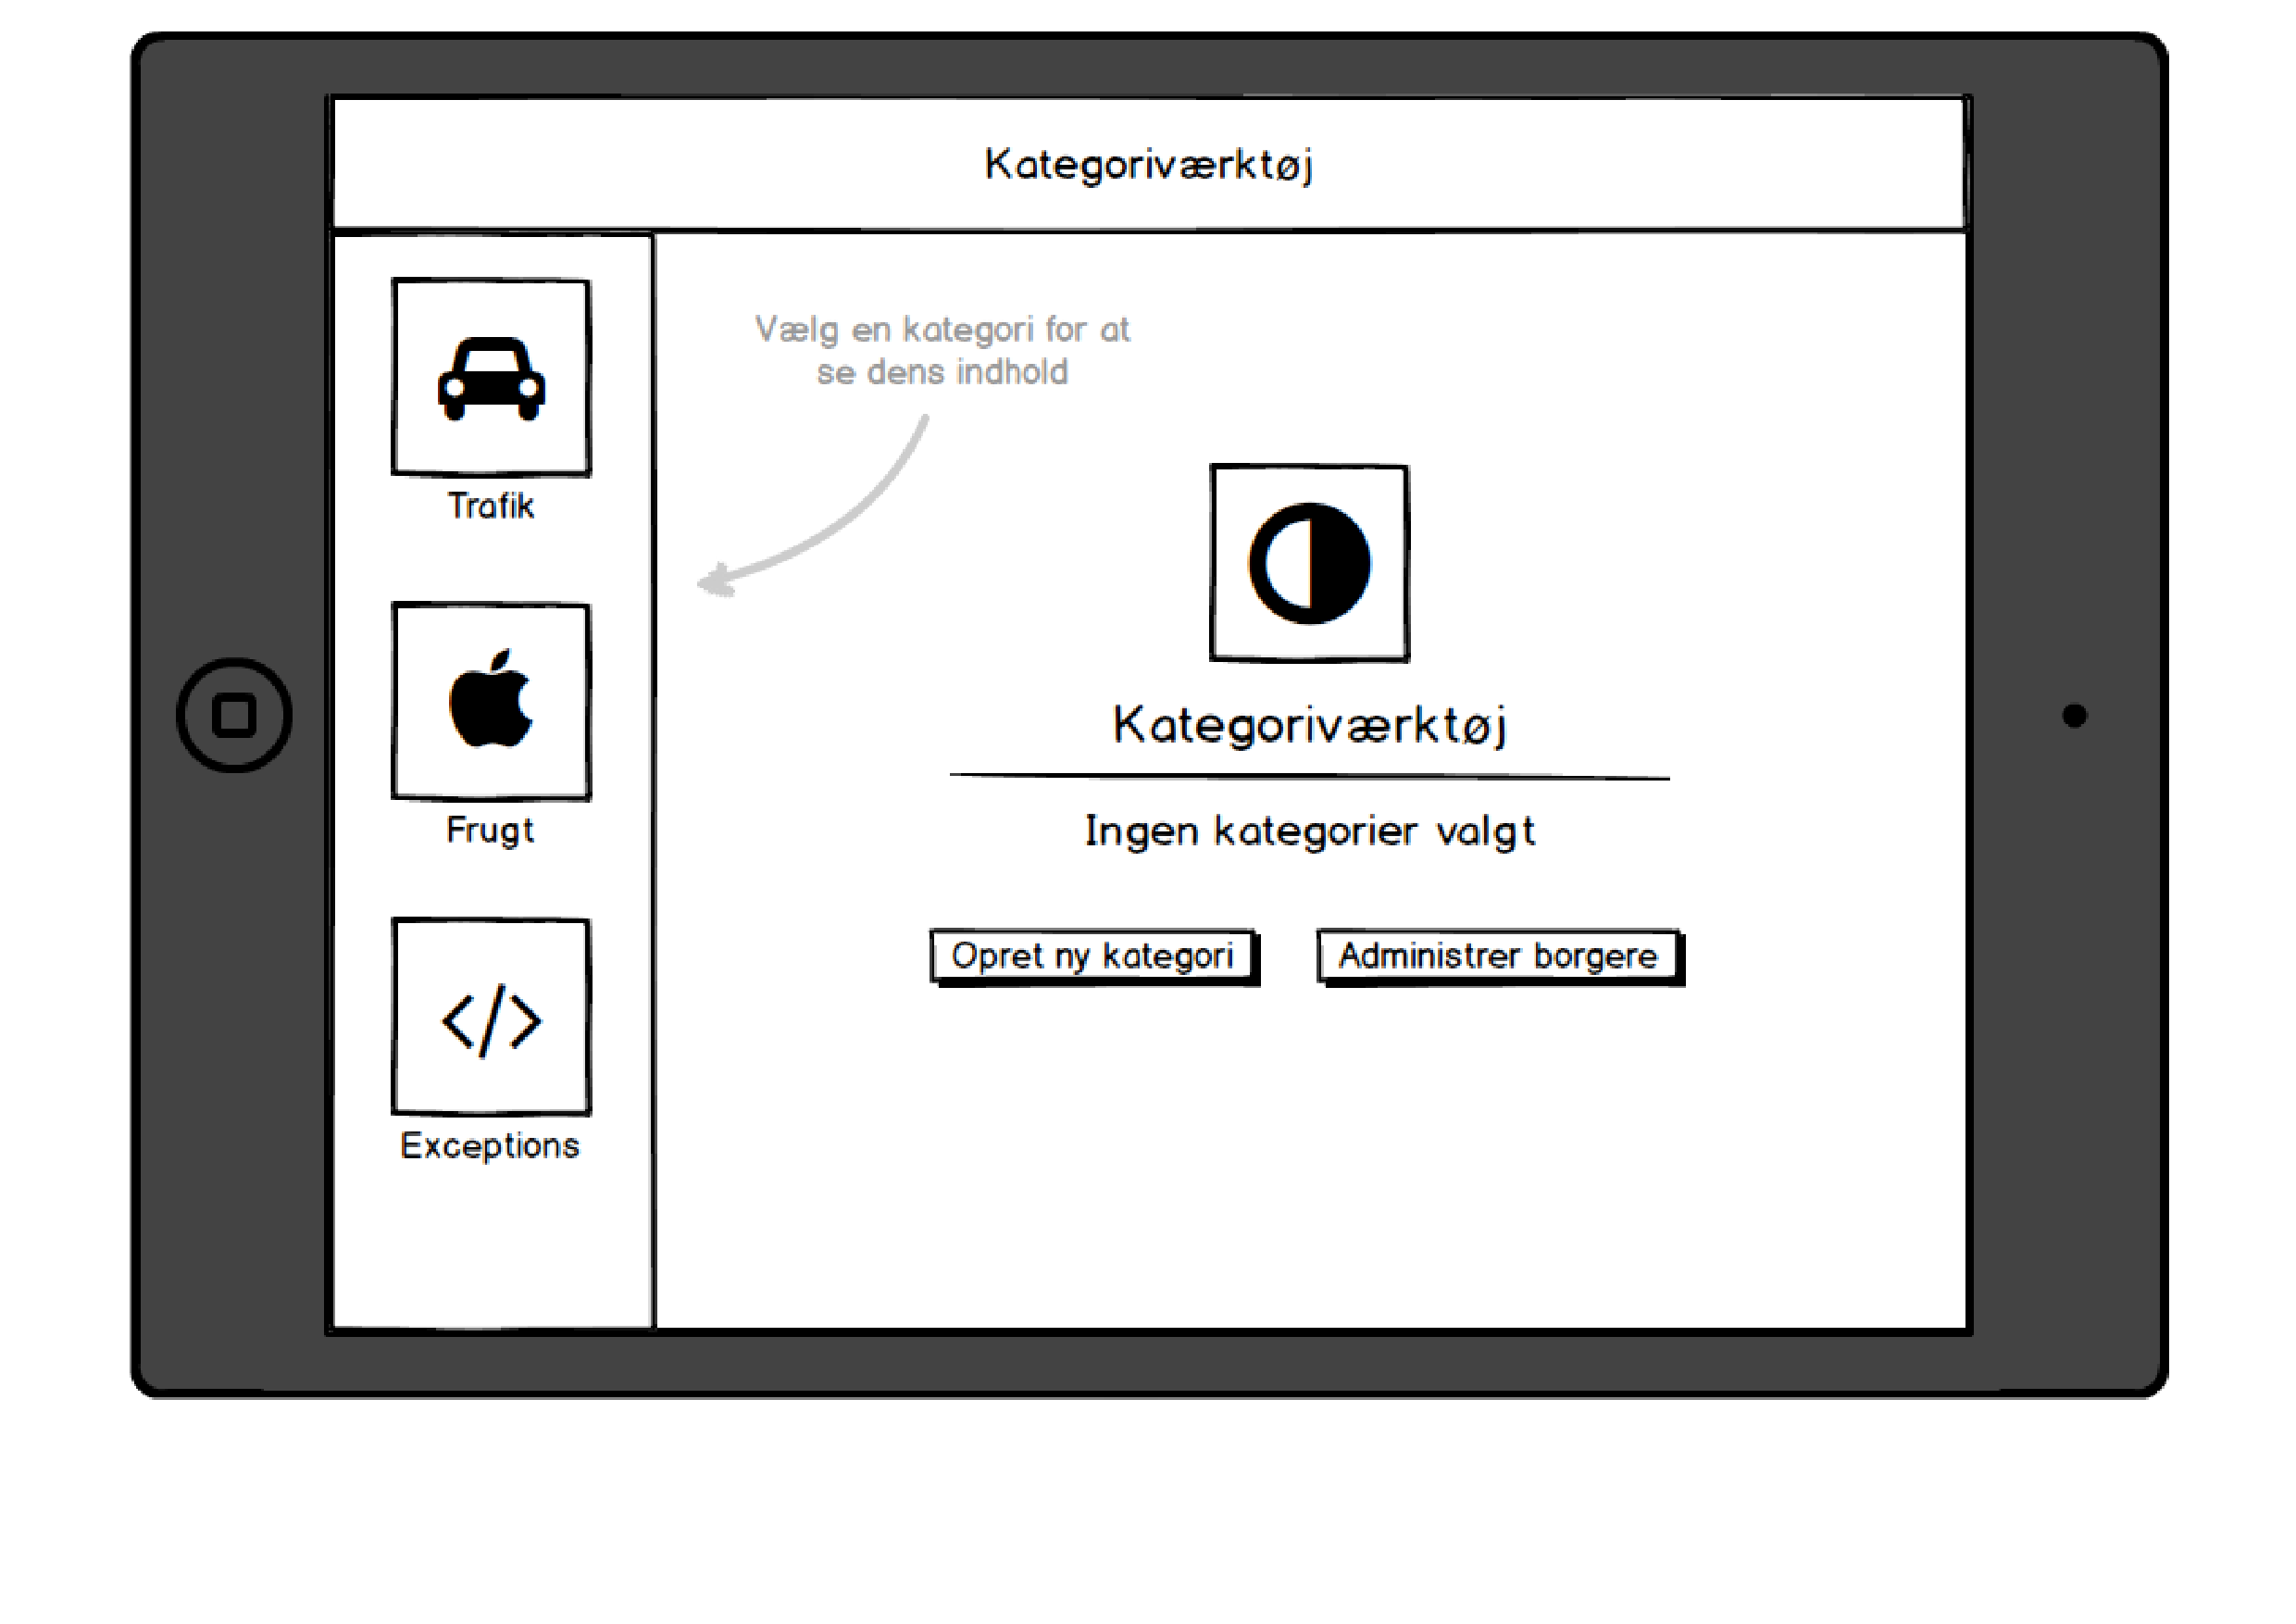
\includegraphics[width=0.75\textwidth]{sprint_two/improved_design/launch_screen}
    \caption{Markup of the home screen}
    \label{fig:improved_design_launch_screen}
\end{figure}

\FloatBarrier

\subsection{Category Selected Screen}
\label{sec:category_selected_screen}
Whenever the user selects a category (in the menu on the left), a screen similar to either \figref{fig:improved_design_category_selected_1} or \figref{fig:improved_design_category_selected_2} should be shown, depending on the presence of pictograms in the category.\\

If the category contains no pictograms, a guide will be shown which will inform the user on how to add pictograms and how to copy the category to citizens. This will inform users on what the different buttons do. However, if the user is new to the system and needs to work on already existing categories, these buttons could possibly be a bit confusing. \\

\begin{figure}[!htbp]
    \centering
    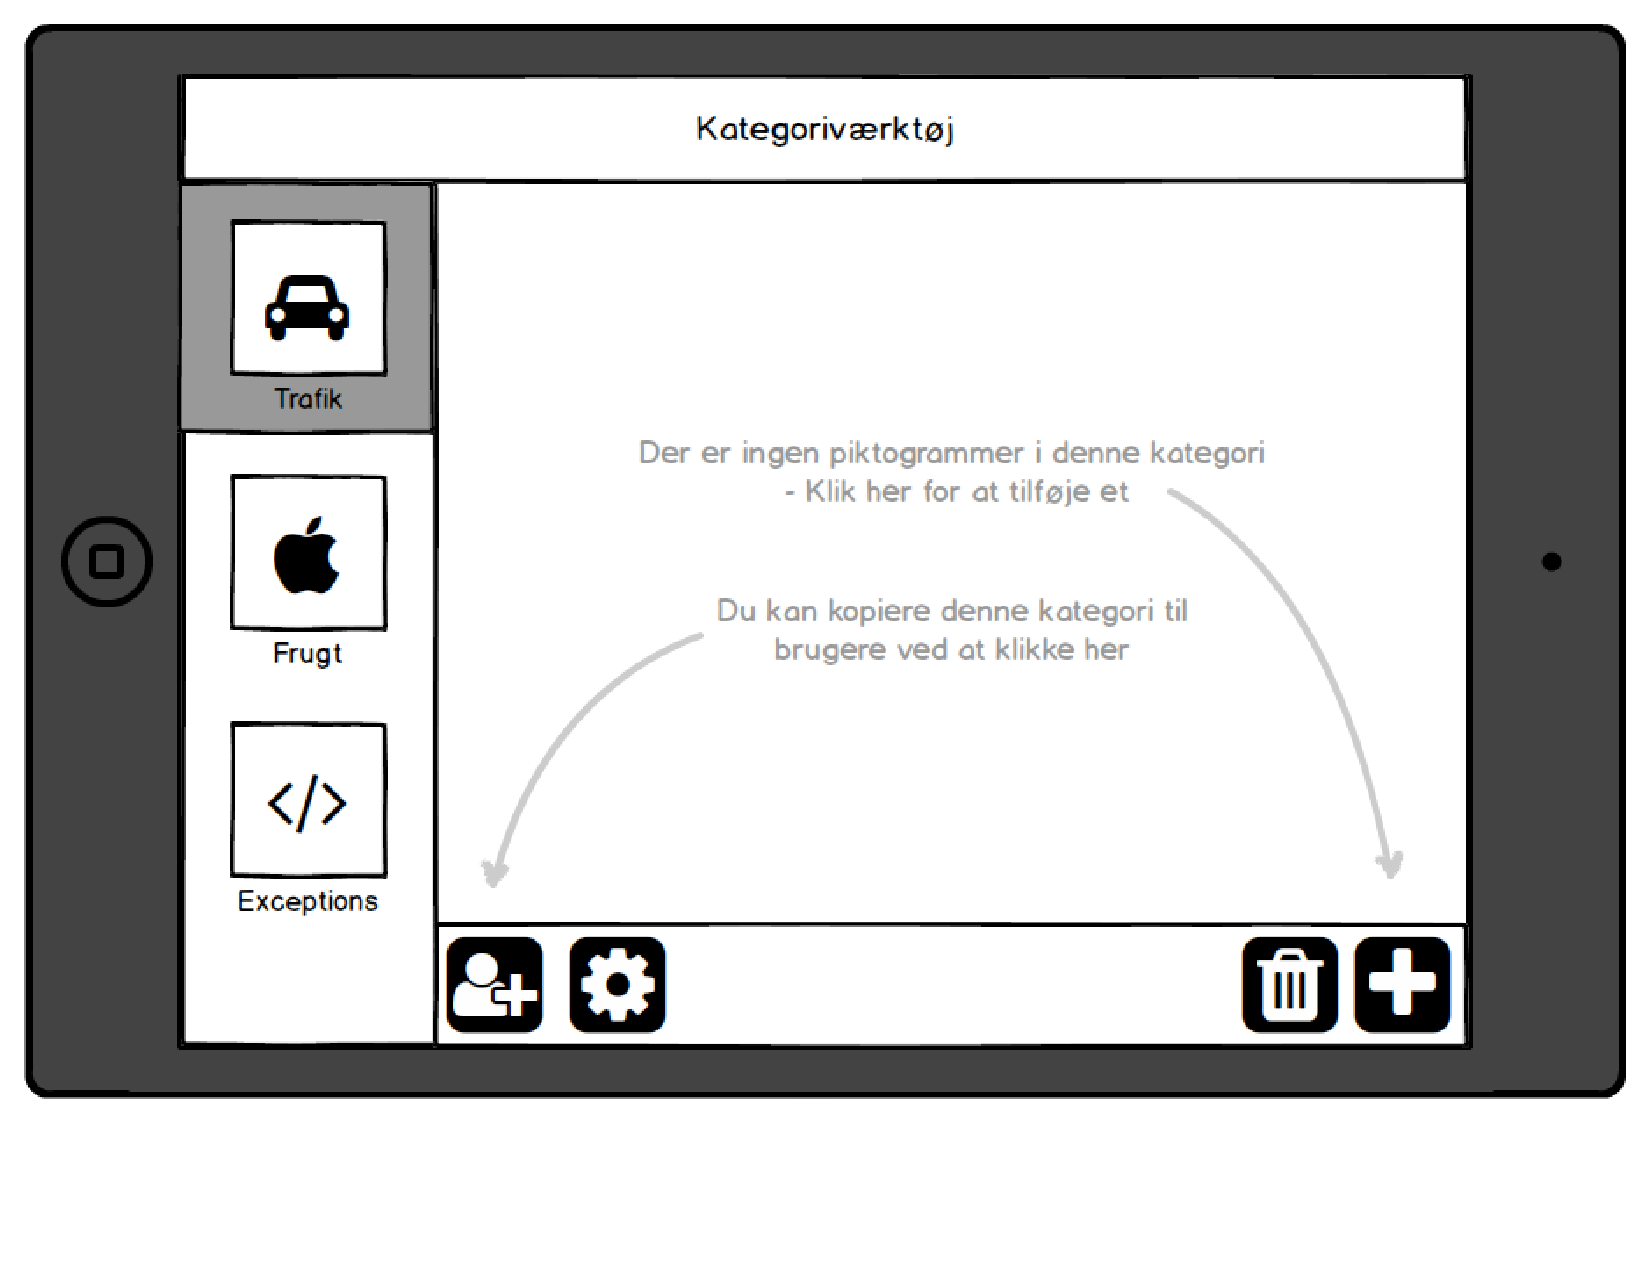
\includegraphics[width=0.75\textwidth]{sprint_two/improved_design/category_selected_1}
    \caption{Markup of the category selected screen without pictograms}
    \label{fig:improved_design_category_selected_1}
\end{figure}

\FloatBarrier

The user will be presented with a screen similar to \figref{fig:improved_design_category_selected_2} if the currently selected category contains pictograms. This screen will present the user with a grid of pictograms in the selected category. The user will be able to scroll through the grid if there are more pictograms than available screen estate. 

\begin{figure}[!htbp]
    \centering
    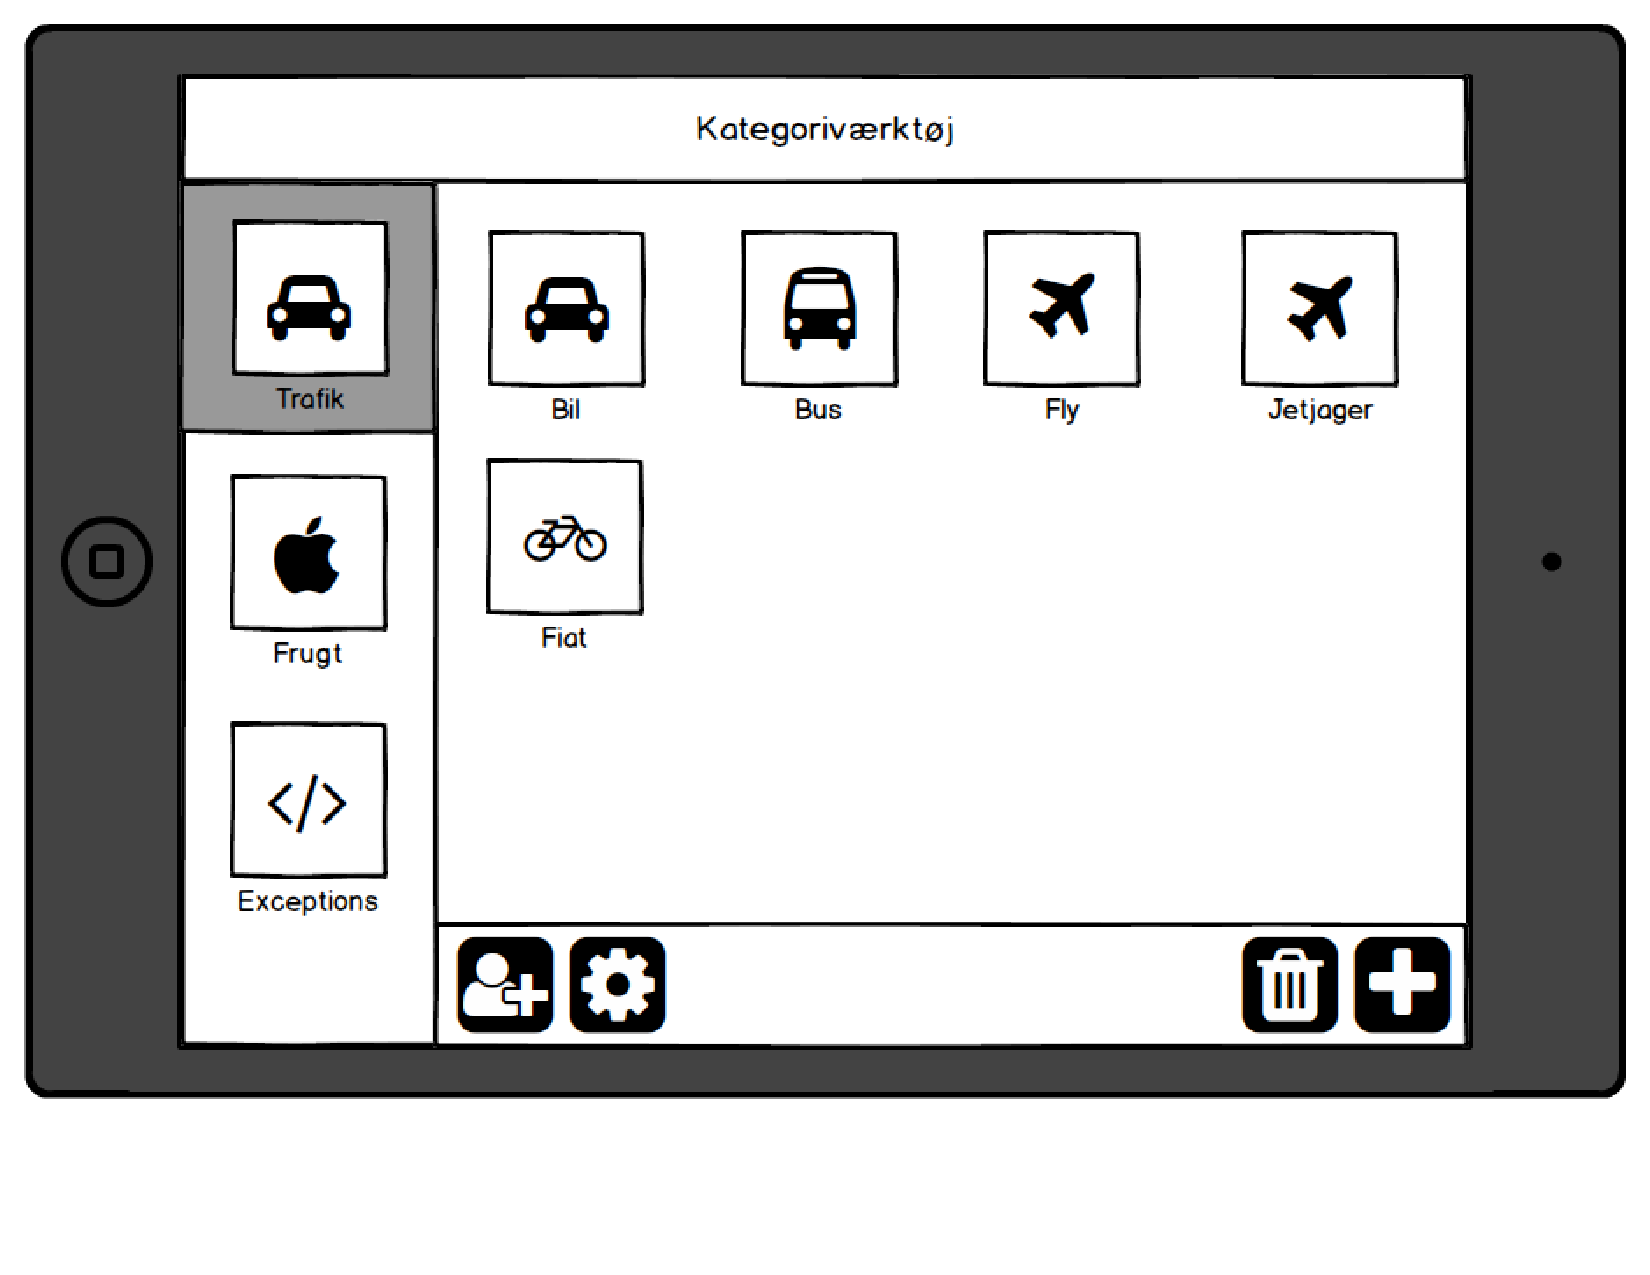
\includegraphics[width=0.75\textwidth]{sprint_two/improved_design/category_selected_2}
    \caption{Markup of the category selected screen with pictograms}
    \label{fig:improved_design_category_selected_2}
\end{figure}

\FloatBarrier

\subsection{Creation and Modification of Categories}
To accommodate the need for creating and removing categories, the following screens have been designed. The category creation screen seen on \figref{fig:improved_design_create_category} will be displayed whenever the \translated{Opret ny kategori}{Create new category} button is pressed on the home screen (see \figref{fig:improved_design_launch_screen}). The point of this screen is to guide the user in the creation of a new category. There are two points to consider when creating a category, namely choosing the eloquent pictogram and title representing the category. To make this clear to the user, two helping arrows have been added, which read \translated{Vælg et piktogram}{Choose a pictogram} and \translated{Skriv en titel}{Write a title}. These arrows have been added so that the user knows that the pictogram-box is clickable and so that it is clear that you are able to write text in the text-box. 

\begin{figure}[!htbp]
    \centering
    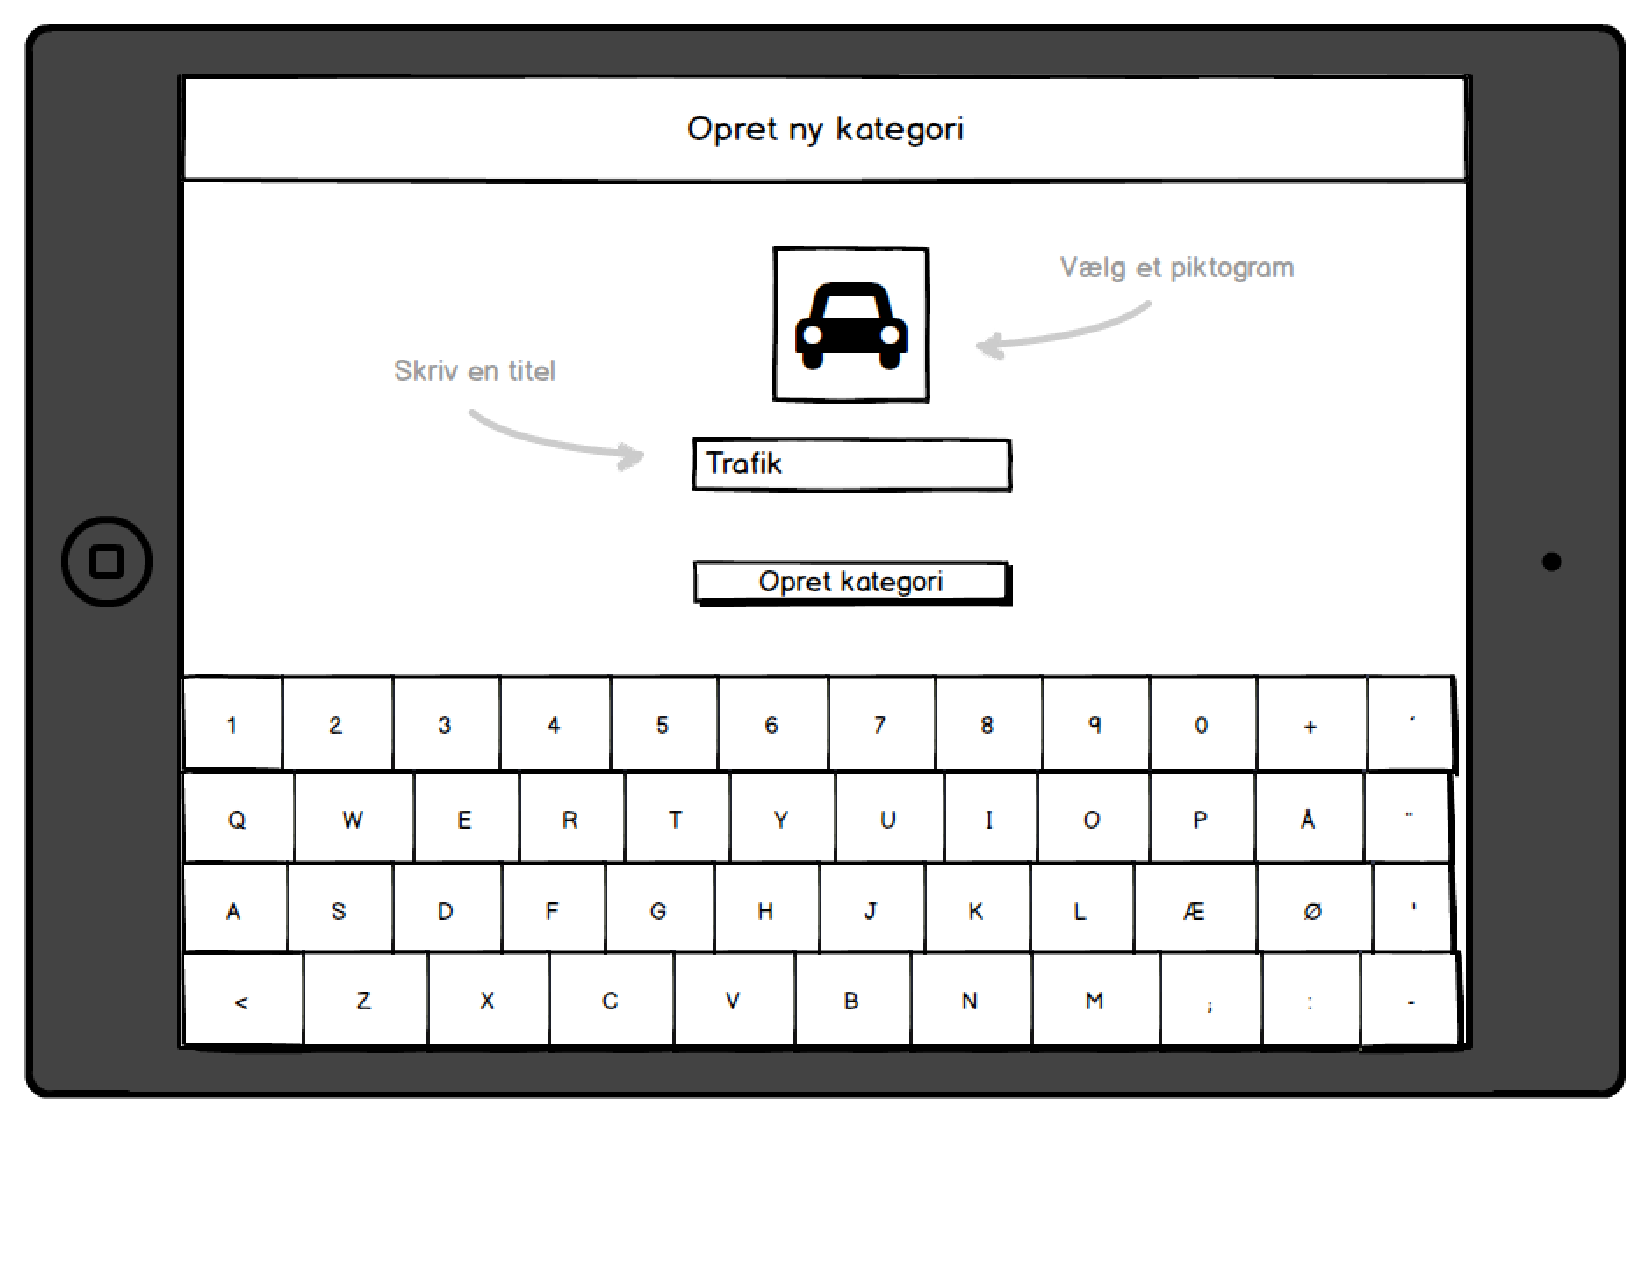
\includegraphics[width=0.75\textwidth]{sprint_two/improved_design/create_category}
    \caption{Markup of the category creation screen}
    \label{fig:improved_design_create_category}
\end{figure}

\FloatBarrier

A user might want to change something regarding a category or deleting a category altogether. To do this, the user must first select a category, then press the cogwheel on the bottom (see \figref{fig:improved_design_category_selected_2}). This will open the dialog-box shown in \figref{fig:improved_design_category_settings}. Here, the user is presented with two buttons, namely \translated{Slet kategori}{Delete category} and \translated{Gem ændringer}{Save changes}. Furthermore, the user is presented with the helpful text \translated{Her kan du ændre piktogrammet og titlen for kategorien}{Here you can change the pictogram and the title for the category}. This dialog does not contain any helpful arrows, because it was deemed unnecessary at this point since the user should be familiar with the way categories are structured. One thing that can be problematic with this design is, that some users might find it hard to figure out how to get this dialog opened. 

\begin{figure}[!htbp]
    \centering
    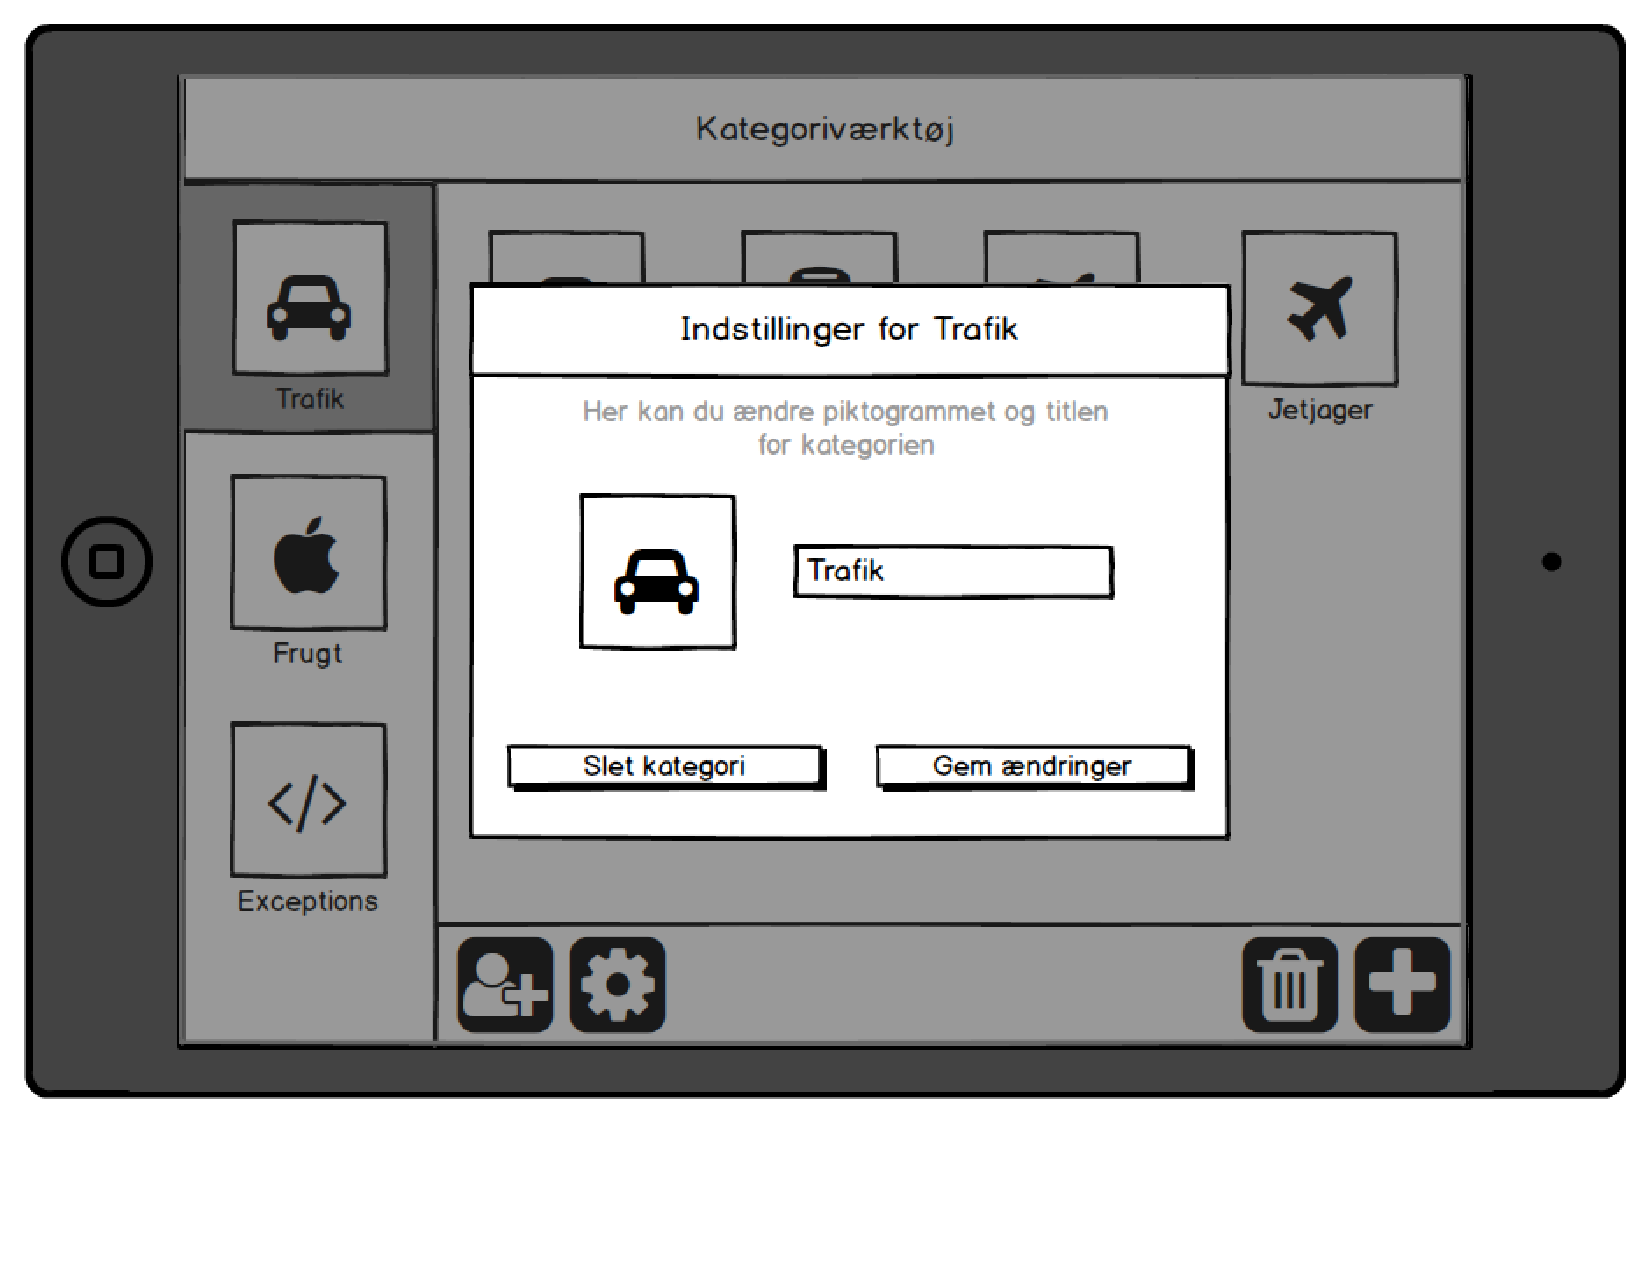
\includegraphics[width=0.75\textwidth]{sprint_two/improved_design/category_settings}
    \caption{Markup of the settings-dialog for a category}
    \label{fig:improved_design_category_settings}
\end{figure}

\FloatBarrier

%!TEX root = ../../../super_main.tex
\section{Implementation of New Design}
\label{sec:implementation_of_new_design}

The implementation of the design from \secref{sec:improved_design} has has been partially implemented during the second sprint. The main goal of second sprint in regards to the \ct was to implement the institute level, where guardians were able to create categories for an entire institution that could later be copied to citizens.\\

As mentioned previously the user is greeted by a homescreen where they can see their current categories or add new ones. This can be seen in \figref{fig:ct_home_screen}. If the user presses the button labeled \translated{Opret ny kategori}{Create new category}, the user is able to create a new category which will be placed in the list on the left. 

\begin{figure}[!htbp]
    \centering
    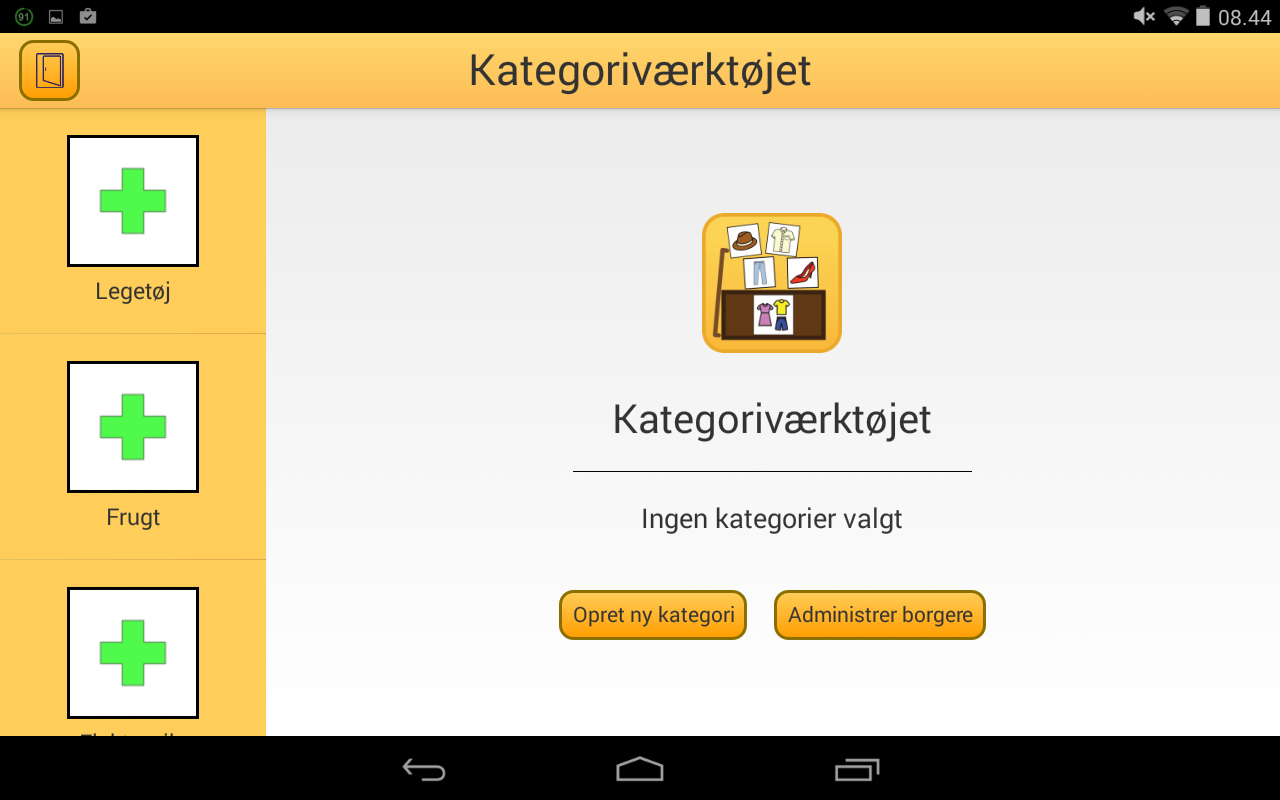
\includegraphics[width=0.75\textwidth]{sprint_two/implementation_of_new_design/homescreen}
    \caption{\ct home screen}
    \label{fig:ct_home_screen}
\end{figure}

If the user selects a category, the pictogram list for that category will be shown, which can be seen in \figref{fig:ct_category_view}.\\

\begin{figure}[!htbp]
    \centering
    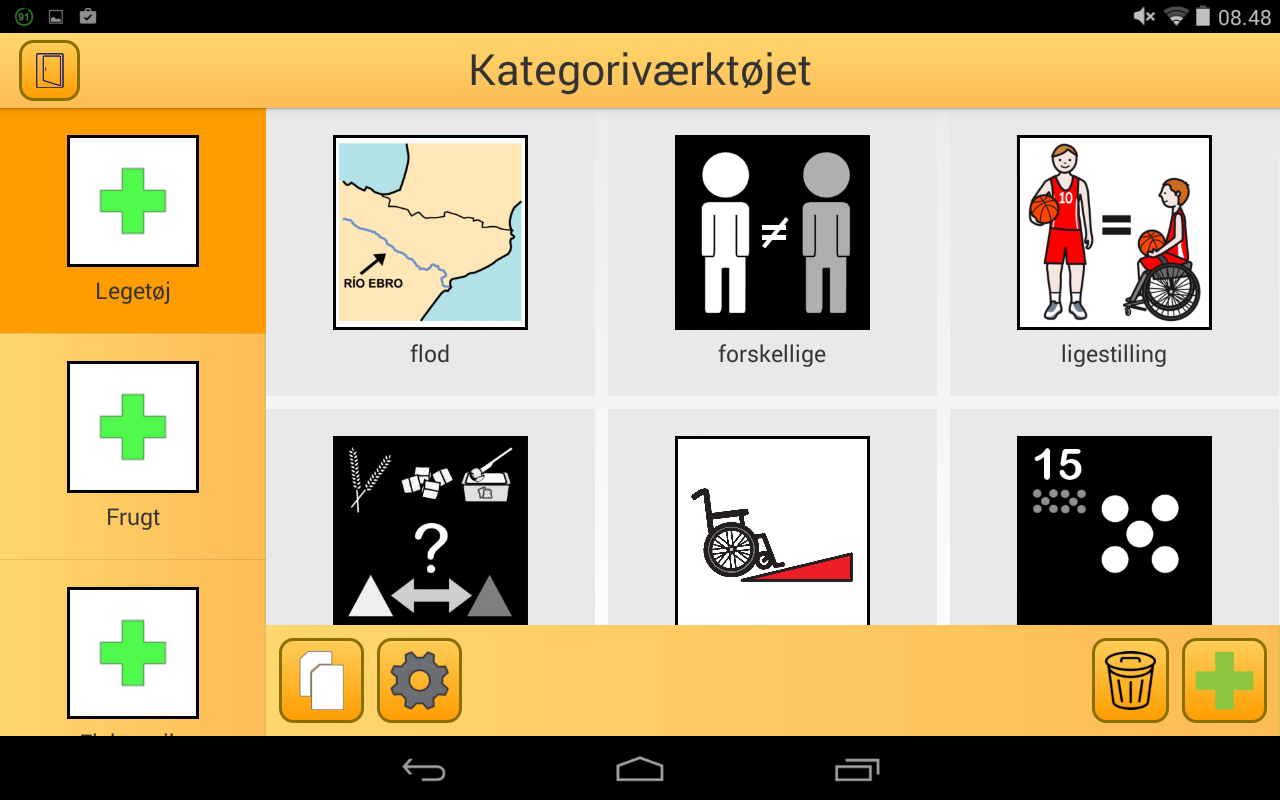
\includegraphics[width=0.75\textwidth]{sprint_two/implementation_of_new_design/categoryview}
    \caption{\ct category selected screen}
    \label{fig:ct_category_view}
\end{figure}


Both the list of categories as well as the list containing pictograms related to the category have been implemented using \mono{ListView}s and Adapters, which makes sure that items in the list are only loaded when the users scroll past it. This makes sure that excessive amounts of memory will not be used to store the complete list of queried categories or pictograms, and thereby make sure that the application does not crash because of lack of memory. \\

The functionality of selecting a pictogram in a category has been implemented, but the visual cue that tells the user which pictogram is selected (as can be seen on the ``Leget\o j'' category in \figref{fig:ct_category_view}) has not currently been implemented. Furthermore the possibility of removing a selected pictogram from category by clicking the Trashcan-icon in the contextual menu at the bottom has also been implemented. Since the \ct-project is not done yet, work on the project will have to be continued on a later point. 


%!TEX root = ../../super_main.tex

\chapter{Sprint Conclusion}
\label{cha:conclusion_sprint_2}

The functionality of selecting a pictogram in a category has been implemented, but the visual cue that tells the user which pictogram is selected (as can be seen on the ``Leget\o j'' category in \figrefpage{fig:ct_category_view}) has not currently been implemented. Furthermore, the possibility of removing a selected pictogram from category by clicking the Trashcan-icon in the contextual menu at the bottom has also been implemented. Since the \ct-project is not done yet, work on the project will have to be continued.
\\\\
The design, complete with mock-ups, and most of the implementation of the graphical user interface of the \ct was completed. Some of the functionality of \ct and some communication with the database was not yet completed. The \ct is ready for implementation of its remaining functionality. The \gc-library was extended with \androidinline{GirafActivity}, a standardized action bar, and various dialogs.